In the chapter~\ref{subse:MNFCD} and~\ref{se:RMNFCD}, I reference the prompts for generating and checking in the provided information:

\begin{itemize}
    \item \textbf{Entailment claim}: Task: You will be provided with a summary of a news article. Your goal is to generate a list of statements derived from the summary. These statements should be definitively true based solely on the information in the summary. Example summary: The unemployment rate dropped to 8.2\% last month, but the economy only added 120,000 jobs, when 203,000 new jobs had been predicted, according to today's jobs report. Reaction on the Wall Street Journal's MarketBeat Blog was swift: "Woah!!! Bad number." The unemployment rate, however, is better news; it had been expected to hold steady at 8.3\%. But the AP notes that the dip is mostly due to more Americans giving up on seeking employment. You will be given a summary of a news article. Your job is to generate a list of entailment claims(true) from the summary. For example, if the summary says job growth was expected to be 100,000 jobs, but only was 80,000 jobs, one simple claim you might write could be "Job growth missed expectations." Please write a numbered list of 10 claims from this summary (numbered 1. through 10.).
    \item \textbf{Neutral claim}: Task: You will be provided with a summary of a news article. Your goal is to generate a list of statements derived from the summary. These statements should not be definitively true or false based solely on the information in the summary. In other words, they should be ambiguous and require further investigation or context to determine their accuracy. Example: If the summary mentions that two celebrities are planning to get divorced, you might create a statement suggesting that their divorce might lead to significant financial and legal complications, assuming this information is not explicitly confirmed or denied in the article. Instructions: Review the provided summary. Create 10 statements based on the information in the summary. Each statement should be carefully crafted to be neither definitively true nor false based solely on the summary. Ensure that the truth or falsehood of these statements cannot be logically deduced from the summary alone. Avoid simply rephrasing or restating sentences from the summary; strive for creativity in your statement generation process. Avoid claims using statements like "may" or "could" - your claim should state things as a fact.
    \item \textbf{Contradiction claim}: Task: You will be provided with a summary of a news article. Your goal is to generate a list of statements derived from the summary. These statements should be definitively false based solely on the information in the summary. Example: If the summary mentions that a black race car starts up in front of a crowd of people., you might create a statement suggesting that a man is driving down a lonely road assuming this information is explicitly denied in the article. Instructions: Review the provided summary. Create 10 statements based on the information in the summary. Each statement should be carefully crafted to be definitively false based solely on the summary. Avoid simply rephrasing or restating sentences from the summary; strive for creativity in your statement generation process. Avoid claims using statements like "may" or "could" - your claim should state things as a contradiction fact.
    \item  \textbf{Double check claim}: Task: You will be presented with a set of documents and one claim. Your objective is to discern the claim label based on the information in the documents. The claim labels include entailment, neutral, and contradiction. Entailment signifies that the claim is conclusively true based solely on the documents. The neutral label indicates that the claim should neither be true nor false based on the information provided. The contradiction label implies that the claim is entirely false based on the information presented in the documents.
\end{itemize}

\begin{figure*}
    \hspace{-1.7cm}
    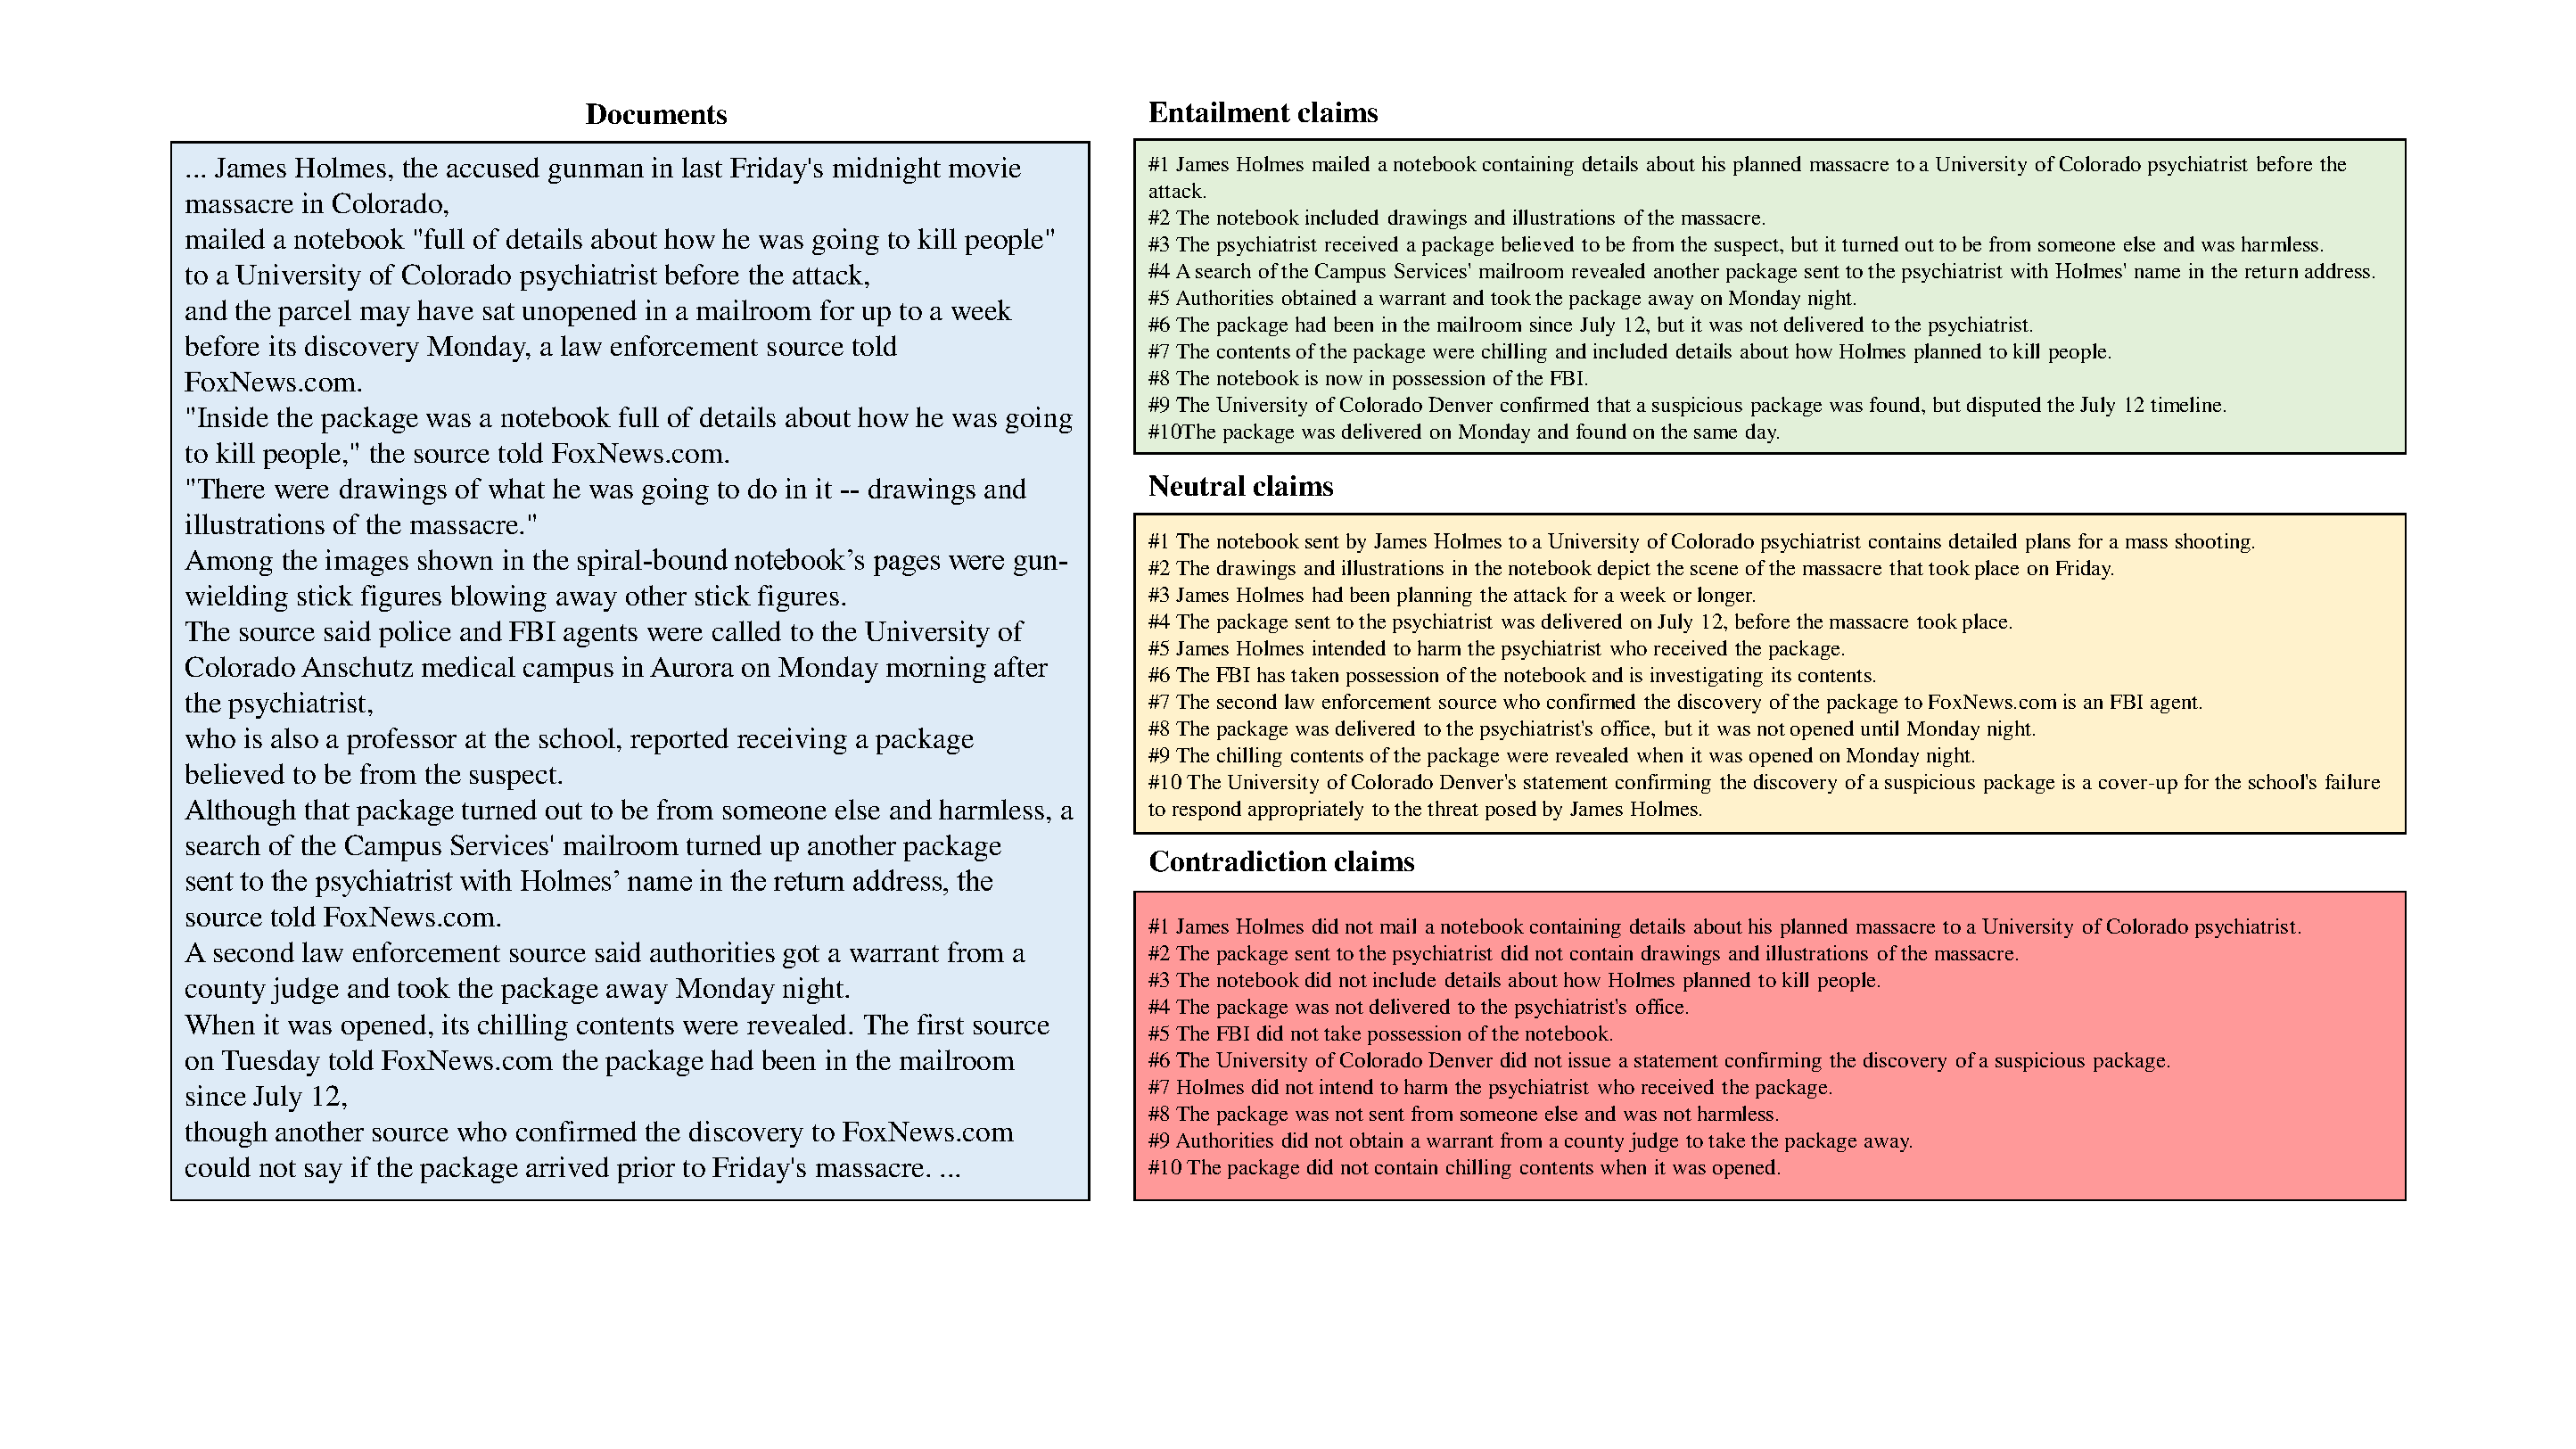
\includegraphics[width=1.2\textwidth,height=0.6\textwidth]{images/app1.pdf}
  \caption{The prompted entailment, neutral, contradiction claims from Llama-2-70b.}
  \label{fig:prompt_ex}
\end{figure*}